\chapter{Revisão bibliográfica}
\label{cap:Revisao_bibliografica_init}

Existem várias formas de se medir a atitude, porém, 
a forma mais amplamente utilizada em satélites de grande porte são os seguidores de estrelas (\textit{star trackers}). 
A tecnologia de tais sistemas vêm evoluindo nos últimos anos, com a rápida melhoria dos sensores CCD (\textit{charge-coupled device}), 
e tecnologias de análise de imagem. Porém,  erros são  inerentes a qualquer medida, por mais pequeno que um erro possa ser, pode levar a uma identificação errônea de uma estrela, resultado em um erro completo de posicionamento.

Star Trackers funcionam capturando imagens de estrelas e comparando a tabelas salvas em memória ~\cite[]{Diaz}. Desta forma, o satélite é capaz de identificar a sua atitude.

No entanto, os sistemas comerciais possuem preço elevado, consumo de energia elevado e massa elevada para pequenos satélites, como é mostrado na Figura ~\ref{fig:Comp_star_trackers_comerciais}.

\begin{figure}[!h]
	\centering
	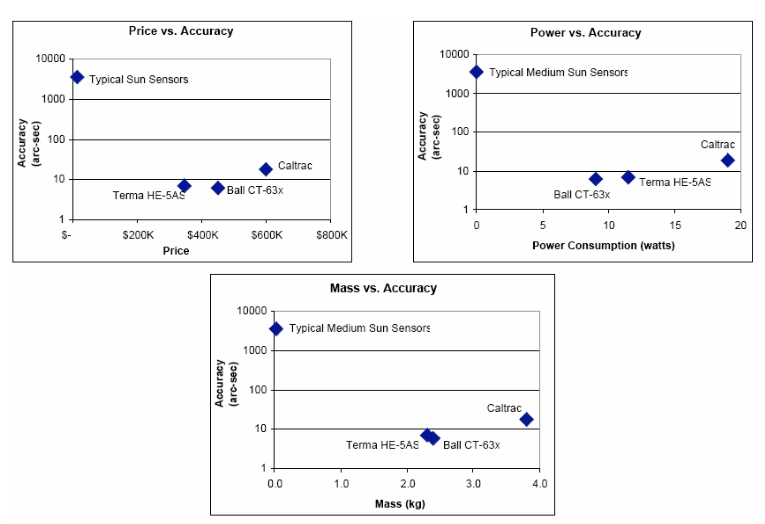
\includegraphics[width=1\columnwidth]{images/comp_star_trackers.png}
	\caption{Comparação de Star Trackers comerciais. (a) Relação entre preço e precisão, (b) Relação entre energia consumida e precisão, (c) Relação entre massa e precisão. Fonte: ~\cite[]{Diaz}}
	\label{fig:Comp_star_trackers_comerciais}
\end{figure}
